\documentclass[UTF8]{ctexart}
\usepackage{graphicx}
\usepackage{enumerate}
\title{EI339 Class Project Report}
\author{陈子轩 516030910545}
\date{2018年12月}

\begin{document}
\maketitle
\tableofcontents
\section{问题描述}
\subsection{股价变动机制}
\begin{figure}[!htbp]
\centering
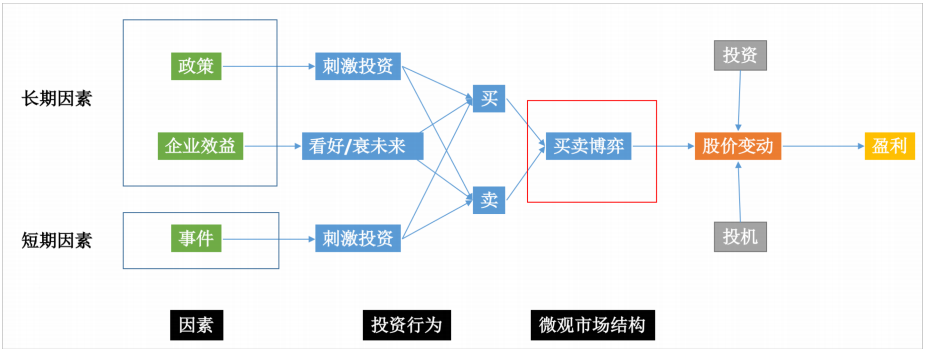
\includegraphics[scale = 0.6]{p1.png}
\caption{股价变动机制}
\end{figure}
如图所示,影响股价变动的机制有长期因素和短期因素,他们都最终归结为买卖博弈来影响价格。买卖博弈可以通过三个方面体现:已公开的买卖需求、正在实施的买卖动作、持币观望。已公开的买卖需求可以通过订单簿来体现,正在实施的买卖动作经研究可以看做是随机尝试的实现,而第三类信息是难以获得的。本次大作业主要研究订单簿对价格的影响。
\subsection{数据描述}
订单簿的数据为:
\begin{enumerate}[*]
    \item 日期(Date)
    \item 时间(Time)
    \item 申买价(Bid Price)
    \item 申买量(Bid Volume)
    \item 申卖价(Ask Price)
    \item 申卖量(Ask Volume)
    \item 最新成交价(Last Price)
    \item 中间价(MidPrice = (Bid Price + Ask Price) / 2)
    \item 当前累计成交数量(Volume)
\end{enumerate}
通过对订单簿中数据的学习,预测下20个时间点中间价(mid price)的均值
\section{算法设计}
\subsection{LSTM}
\subsubsection{算法介绍}
\subsubsection{建模方式}
\subsubsection{参数选择依据}
\subsection{DNN}
\subsubsection{算法介绍}
\subsubsection{建模方式}
\subsection{其他的尝试——底层LSTM的实现}
\subsubsection{模型搭建的方法}
\section{组员分工}
\section{感想}
\section{参考文献}

\end{document}